% !TEX root = final_report.tex
%
%  PACKAGE IMPORTS
%
\documentclass{article} % For LaTeX2e
\usepackage{iclr2022_conference,times}
%%%%% NEW MATH DEFINITIONS %%%%%

\usepackage{amsmath,amsfonts,bm}

% Mark sections of captions for referring to divisions of figures
\newcommand{\figleft}{{\em (Left)}}
\newcommand{\figcenter}{{\em (Center)}}
\newcommand{\figright}{{\em (Right)}}
\newcommand{\figtop}{{\em (Top)}}
\newcommand{\figbottom}{{\em (Bottom)}}
\newcommand{\captiona}{{\em (a)}}
\newcommand{\captionb}{{\em (b)}}
\newcommand{\captionc}{{\em (c)}}
\newcommand{\captiond}{{\em (d)}}

% Highlight a newly defined term
\newcommand{\newterm}[1]{{\bf #1}}


% Figure reference, lower-case.
\def\figref#1{figure~\ref{#1}}
% Figure reference, capital. For start of sentence
\def\Figref#1{Figure~\ref{#1}}
\def\twofigref#1#2{figures \ref{#1} and \ref{#2}}
\def\quadfigref#1#2#3#4{figures \ref{#1}, \ref{#2}, \ref{#3} and \ref{#4}}
% Section reference, lower-case.
\def\secref#1{section~\ref{#1}}
% Section reference, capital.
\def\Secref#1{Section~\ref{#1}}
% Reference to two sections.
\def\twosecrefs#1#2{sections \ref{#1} and \ref{#2}}
% Reference to three sections.
\def\secrefs#1#2#3{sections \ref{#1}, \ref{#2} and \ref{#3}}
% Reference to an equation, lower-case.
\def\eqref#1{equation~\ref{#1}}
% Reference to an equation, upper case
\def\Eqref#1{Equation~\ref{#1}}
% A raw reference to an equation---avoid using if possible
\def\plaineqref#1{\ref{#1}}
% Reference to a chapter, lower-case.
\def\chapref#1{chapter~\ref{#1}}
% Reference to an equation, upper case.
\def\Chapref#1{Chapter~\ref{#1}}
% Reference to a range of chapters
\def\rangechapref#1#2{chapters\ref{#1}--\ref{#2}}
% Reference to an algorithm, lower-case.
\def\algref#1{algorithm~\ref{#1}}
% Reference to an algorithm, upper case.
\def\Algref#1{Algorithm~\ref{#1}}
\def\twoalgref#1#2{algorithms \ref{#1} and \ref{#2}}
\def\Twoalgref#1#2{Algorithms \ref{#1} and \ref{#2}}
% Reference to a part, lower case
\def\partref#1{part~\ref{#1}}
% Reference to a part, upper case
\def\Partref#1{Part~\ref{#1}}
\def\twopartref#1#2{parts \ref{#1} and \ref{#2}}

\def\ceil#1{\lceil #1 \rceil}
\def\floor#1{\lfloor #1 \rfloor}
\def\1{\bm{1}}
\newcommand{\train}{\mathcal{D}}
\newcommand{\valid}{\mathcal{D_{\mathrm{valid}}}}
\newcommand{\test}{\mathcal{D_{\mathrm{test}}}}

\def\eps{{\epsilon}}


% Random variables
\def\reta{{\textnormal{$\eta$}}}
\def\ra{{\textnormal{a}}}
\def\rb{{\textnormal{b}}}
\def\rc{{\textnormal{c}}}
\def\rd{{\textnormal{d}}}
\def\re{{\textnormal{e}}}
\def\rf{{\textnormal{f}}}
\def\rg{{\textnormal{g}}}
\def\rh{{\textnormal{h}}}
\def\ri{{\textnormal{i}}}
\def\rj{{\textnormal{j}}}
\def\rk{{\textnormal{k}}}
\def\rl{{\textnormal{l}}}
% rm is already a command, just don't name any random variables m
\def\rn{{\textnormal{n}}}
\def\ro{{\textnormal{o}}}
\def\rp{{\textnormal{p}}}
\def\rq{{\textnormal{q}}}
\def\rr{{\textnormal{r}}}
\def\rs{{\textnormal{s}}}
\def\rt{{\textnormal{t}}}
\def\ru{{\textnormal{u}}}
\def\rv{{\textnormal{v}}}
\def\rw{{\textnormal{w}}}
\def\rx{{\textnormal{x}}}
\def\ry{{\textnormal{y}}}
\def\rz{{\textnormal{z}}}

% Random vectors
\def\rvepsilon{{\mathbf{\epsilon}}}
\def\rvtheta{{\mathbf{\theta}}}
\def\rva{{\mathbf{a}}}
\def\rvb{{\mathbf{b}}}
\def\rvc{{\mathbf{c}}}
\def\rvd{{\mathbf{d}}}
\def\rve{{\mathbf{e}}}
\def\rvf{{\mathbf{f}}}
\def\rvg{{\mathbf{g}}}
\def\rvh{{\mathbf{h}}}
\def\rvu{{\mathbf{i}}}
\def\rvj{{\mathbf{j}}}
\def\rvk{{\mathbf{k}}}
\def\rvl{{\mathbf{l}}}
\def\rvm{{\mathbf{m}}}
\def\rvn{{\mathbf{n}}}
\def\rvo{{\mathbf{o}}}
\def\rvp{{\mathbf{p}}}
\def\rvq{{\mathbf{q}}}
\def\rvr{{\mathbf{r}}}
\def\rvs{{\mathbf{s}}}
\def\rvt{{\mathbf{t}}}
\def\rvu{{\mathbf{u}}}
\def\rvv{{\mathbf{v}}}
\def\rvw{{\mathbf{w}}}
\def\rvx{{\mathbf{x}}}
\def\rvy{{\mathbf{y}}}
\def\rvz{{\mathbf{z}}}

% Elements of random vectors
\def\erva{{\textnormal{a}}}
\def\ervb{{\textnormal{b}}}
\def\ervc{{\textnormal{c}}}
\def\ervd{{\textnormal{d}}}
\def\erve{{\textnormal{e}}}
\def\ervf{{\textnormal{f}}}
\def\ervg{{\textnormal{g}}}
\def\ervh{{\textnormal{h}}}
\def\ervi{{\textnormal{i}}}
\def\ervj{{\textnormal{j}}}
\def\ervk{{\textnormal{k}}}
\def\ervl{{\textnormal{l}}}
\def\ervm{{\textnormal{m}}}
\def\ervn{{\textnormal{n}}}
\def\ervo{{\textnormal{o}}}
\def\ervp{{\textnormal{p}}}
\def\ervq{{\textnormal{q}}}
\def\ervr{{\textnormal{r}}}
\def\ervs{{\textnormal{s}}}
\def\ervt{{\textnormal{t}}}
\def\ervu{{\textnormal{u}}}
\def\ervv{{\textnormal{v}}}
\def\ervw{{\textnormal{w}}}
\def\ervx{{\textnormal{x}}}
\def\ervy{{\textnormal{y}}}
\def\ervz{{\textnormal{z}}}

% Random matrices
\def\rmA{{\mathbf{A}}}
\def\rmB{{\mathbf{B}}}
\def\rmC{{\mathbf{C}}}
\def\rmD{{\mathbf{D}}}
\def\rmE{{\mathbf{E}}}
\def\rmF{{\mathbf{F}}}
\def\rmG{{\mathbf{G}}}
\def\rmH{{\mathbf{H}}}
\def\rmI{{\mathbf{I}}}
\def\rmJ{{\mathbf{J}}}
\def\rmK{{\mathbf{K}}}
\def\rmL{{\mathbf{L}}}
\def\rmM{{\mathbf{M}}}
\def\rmN{{\mathbf{N}}}
\def\rmO{{\mathbf{O}}}
\def\rmP{{\mathbf{P}}}
\def\rmQ{{\mathbf{Q}}}
\def\rmR{{\mathbf{R}}}
\def\rmS{{\mathbf{S}}}
\def\rmT{{\mathbf{T}}}
\def\rmU{{\mathbf{U}}}
\def\rmV{{\mathbf{V}}}
\def\rmW{{\mathbf{W}}}
\def\rmX{{\mathbf{X}}}
\def\rmY{{\mathbf{Y}}}
\def\rmZ{{\mathbf{Z}}}

% Elements of random matrices
\def\ermA{{\textnormal{A}}}
\def\ermB{{\textnormal{B}}}
\def\ermC{{\textnormal{C}}}
\def\ermD{{\textnormal{D}}}
\def\ermE{{\textnormal{E}}}
\def\ermF{{\textnormal{F}}}
\def\ermG{{\textnormal{G}}}
\def\ermH{{\textnormal{H}}}
\def\ermI{{\textnormal{I}}}
\def\ermJ{{\textnormal{J}}}
\def\ermK{{\textnormal{K}}}
\def\ermL{{\textnormal{L}}}
\def\ermM{{\textnormal{M}}}
\def\ermN{{\textnormal{N}}}
\def\ermO{{\textnormal{O}}}
\def\ermP{{\textnormal{P}}}
\def\ermQ{{\textnormal{Q}}}
\def\ermR{{\textnormal{R}}}
\def\ermS{{\textnormal{S}}}
\def\ermT{{\textnormal{T}}}
\def\ermU{{\textnormal{U}}}
\def\ermV{{\textnormal{V}}}
\def\ermW{{\textnormal{W}}}
\def\ermX{{\textnormal{X}}}
\def\ermY{{\textnormal{Y}}}
\def\ermZ{{\textnormal{Z}}}

% Vectors
\def\vzero{{\bm{0}}}
\def\vone{{\bm{1}}}
\def\vmu{{\bm{\mu}}}
\def\vtheta{{\bm{\theta}}}
\def\va{{\bm{a}}}
\def\vb{{\bm{b}}}
\def\vc{{\bm{c}}}
\def\vd{{\bm{d}}}
\def\ve{{\bm{e}}}
\def\vf{{\bm{f}}}
\def\vg{{\bm{g}}}
\def\vh{{\bm{h}}}
\def\vi{{\bm{i}}}
\def\vj{{\bm{j}}}
\def\vk{{\bm{k}}}
\def\vl{{\bm{l}}}
\def\vm{{\bm{m}}}
\def\vn{{\bm{n}}}
\def\vo{{\bm{o}}}
\def\vp{{\bm{p}}}
\def\vq{{\bm{q}}}
\def\vr{{\bm{r}}}
\def\vs{{\bm{s}}}
\def\vt{{\bm{t}}}
\def\vu{{\bm{u}}}
\def\vv{{\bm{v}}}
\def\vw{{\bm{w}}}
\def\vx{{\bm{x}}}
\def\vy{{\bm{y}}}
\def\vz{{\bm{z}}}

% Elements of vectors
\def\evalpha{{\alpha}}
\def\evbeta{{\beta}}
\def\evepsilon{{\epsilon}}
\def\evlambda{{\lambda}}
\def\evomega{{\omega}}
\def\evmu{{\mu}}
\def\evpsi{{\psi}}
\def\evsigma{{\sigma}}
\def\evtheta{{\theta}}
\def\eva{{a}}
\def\evb{{b}}
\def\evc{{c}}
\def\evd{{d}}
\def\eve{{e}}
\def\evf{{f}}
\def\evg{{g}}
\def\evh{{h}}
\def\evi{{i}}
\def\evj{{j}}
\def\evk{{k}}
\def\evl{{l}}
\def\evm{{m}}
\def\evn{{n}}
\def\evo{{o}}
\def\evp{{p}}
\def\evq{{q}}
\def\evr{{r}}
\def\evs{{s}}
\def\evt{{t}}
\def\evu{{u}}
\def\evv{{v}}
\def\evw{{w}}
\def\evx{{x}}
\def\evy{{y}}
\def\evz{{z}}

% Matrix
\def\mA{{\bm{A}}}
\def\mB{{\bm{B}}}
\def\mC{{\bm{C}}}
\def\mD{{\bm{D}}}
\def\mE{{\bm{E}}}
\def\mF{{\bm{F}}}
\def\mG{{\bm{G}}}
\def\mH{{\bm{H}}}
\def\mI{{\bm{I}}}
\def\mJ{{\bm{J}}}
\def\mK{{\bm{K}}}
\def\mL{{\bm{L}}}
\def\mM{{\bm{M}}}
\def\mN{{\bm{N}}}
\def\mO{{\bm{O}}}
\def\mP{{\bm{P}}}
\def\mQ{{\bm{Q}}}
\def\mR{{\bm{R}}}
\def\mS{{\bm{S}}}
\def\mT{{\bm{T}}}
\def\mU{{\bm{U}}}
\def\mV{{\bm{V}}}
\def\mW{{\bm{W}}}
\def\mX{{\bm{X}}}
\def\mY{{\bm{Y}}}
\def\mZ{{\bm{Z}}}
\def\mBeta{{\bm{\beta}}}
\def\mPhi{{\bm{\Phi}}}
\def\mLambda{{\bm{\Lambda}}}
\def\mSigma{{\bm{\Sigma}}}

% Tensor
\DeclareMathAlphabet{\mathsfit}{\encodingdefault}{\sfdefault}{m}{sl}
\SetMathAlphabet{\mathsfit}{bold}{\encodingdefault}{\sfdefault}{bx}{n}
\newcommand{\tens}[1]{\bm{\mathsfit{#1}}}
\def\tA{{\tens{A}}}
\def\tB{{\tens{B}}}
\def\tC{{\tens{C}}}
\def\tD{{\tens{D}}}
\def\tE{{\tens{E}}}
\def\tF{{\tens{F}}}
\def\tG{{\tens{G}}}
\def\tH{{\tens{H}}}
\def\tI{{\tens{I}}}
\def\tJ{{\tens{J}}}
\def\tK{{\tens{K}}}
\def\tL{{\tens{L}}}
\def\tM{{\tens{M}}}
\def\tN{{\tens{N}}}
\def\tO{{\tens{O}}}
\def\tP{{\tens{P}}}
\def\tQ{{\tens{Q}}}
\def\tR{{\tens{R}}}
\def\tS{{\tens{S}}}
\def\tT{{\tens{T}}}
\def\tU{{\tens{U}}}
\def\tV{{\tens{V}}}
\def\tW{{\tens{W}}}
\def\tX{{\tens{X}}}
\def\tY{{\tens{Y}}}
\def\tZ{{\tens{Z}}}


% Graph
\def\gA{{\mathcal{A}}}
\def\gB{{\mathcal{B}}}
\def\gC{{\mathcal{C}}}
\def\gD{{\mathcal{D}}}
\def\gE{{\mathcal{E}}}
\def\gF{{\mathcal{F}}}
\def\gG{{\mathcal{G}}}
\def\gH{{\mathcal{H}}}
\def\gI{{\mathcal{I}}}
\def\gJ{{\mathcal{J}}}
\def\gK{{\mathcal{K}}}
\def\gL{{\mathcal{L}}}
\def\gM{{\mathcal{M}}}
\def\gN{{\mathcal{N}}}
\def\gO{{\mathcal{O}}}
\def\gP{{\mathcal{P}}}
\def\gQ{{\mathcal{Q}}}
\def\gR{{\mathcal{R}}}
\def\gS{{\mathcal{S}}}
\def\gT{{\mathcal{T}}}
\def\gU{{\mathcal{U}}}
\def\gV{{\mathcal{V}}}
\def\gW{{\mathcal{W}}}
\def\gX{{\mathcal{X}}}
\def\gY{{\mathcal{Y}}}
\def\gZ{{\mathcal{Z}}}

% Sets
\def\sA{{\mathbb{A}}}
\def\sB{{\mathbb{B}}}
\def\sC{{\mathbb{C}}}
\def\sD{{\mathbb{D}}}
% Don't use a set called E, because this would be the same as our symbol
% for expectation.
\def\sF{{\mathbb{F}}}
\def\sG{{\mathbb{G}}}
\def\sH{{\mathbb{H}}}
\def\sI{{\mathbb{I}}}
\def\sJ{{\mathbb{J}}}
\def\sK{{\mathbb{K}}}
\def\sL{{\mathbb{L}}}
\def\sM{{\mathbb{M}}}
\def\sN{{\mathbb{N}}}
\def\sO{{\mathbb{O}}}
\def\sP{{\mathbb{P}}}
\def\sQ{{\mathbb{Q}}}
\def\sR{{\mathbb{R}}}
\def\sS{{\mathbb{S}}}
\def\sT{{\mathbb{T}}}
\def\sU{{\mathbb{U}}}
\def\sV{{\mathbb{V}}}
\def\sW{{\mathbb{W}}}
\def\sX{{\mathbb{X}}}
\def\sY{{\mathbb{Y}}}
\def\sZ{{\mathbb{Z}}}

% Entries of a matrix
\def\emLambda{{\Lambda}}
\def\emA{{A}}
\def\emB{{B}}
\def\emC{{C}}
\def\emD{{D}}
\def\emE{{E}}
\def\emF{{F}}
\def\emG{{G}}
\def\emH{{H}}
\def\emI{{I}}
\def\emJ{{J}}
\def\emK{{K}}
\def\emL{{L}}
\def\emM{{M}}
\def\emN{{N}}
\def\emO{{O}}
\def\emP{{P}}
\def\emQ{{Q}}
\def\emR{{R}}
\def\emS{{S}}
\def\emT{{T}}
\def\emU{{U}}
\def\emV{{V}}
\def\emW{{W}}
\def\emX{{X}}
\def\emY{{Y}}
\def\emZ{{Z}}
\def\emSigma{{\Sigma}}

% entries of a tensor
% Same font as tensor, without \bm wrapper
\newcommand{\etens}[1]{\mathsfit{#1}}
\def\etLambda{{\etens{\Lambda}}}
\def\etA{{\etens{A}}}
\def\etB{{\etens{B}}}
\def\etC{{\etens{C}}}
\def\etD{{\etens{D}}}
\def\etE{{\etens{E}}}
\def\etF{{\etens{F}}}
\def\etG{{\etens{G}}}
\def\etH{{\etens{H}}}
\def\etI{{\etens{I}}}
\def\etJ{{\etens{J}}}
\def\etK{{\etens{K}}}
\def\etL{{\etens{L}}}
\def\etM{{\etens{M}}}
\def\etN{{\etens{N}}}
\def\etO{{\etens{O}}}
\def\etP{{\etens{P}}}
\def\etQ{{\etens{Q}}}
\def\etR{{\etens{R}}}
\def\etS{{\etens{S}}}
\def\etT{{\etens{T}}}
\def\etU{{\etens{U}}}
\def\etV{{\etens{V}}}
\def\etW{{\etens{W}}}
\def\etX{{\etens{X}}}
\def\etY{{\etens{Y}}}
\def\etZ{{\etens{Z}}}

% The true underlying data generating distribution
\newcommand{\pdata}{p_{\rm{data}}}
% The empirical distribution defined by the training set
\newcommand{\ptrain}{\hat{p}_{\rm{data}}}
\newcommand{\Ptrain}{\hat{P}_{\rm{data}}}
% The model distribution
\newcommand{\pmodel}{p_{\rm{model}}}
\newcommand{\Pmodel}{P_{\rm{model}}}
\newcommand{\ptildemodel}{\tilde{p}_{\rm{model}}}
% Stochastic autoencoder distributions
\newcommand{\pencode}{p_{\rm{encoder}}}
\newcommand{\pdecode}{p_{\rm{decoder}}}
\newcommand{\precons}{p_{\rm{reconstruct}}}

\newcommand{\laplace}{\mathrm{Laplace}} % Laplace distribution

\newcommand{\E}{\mathbb{E}}
\newcommand{\Ls}{\mathcal{L}}
\newcommand{\R}{\mathbb{R}}
\newcommand{\emp}{\tilde{p}}
\newcommand{\lr}{\alpha}
\newcommand{\reg}{\lambda}
\newcommand{\rect}{\mathrm{rectifier}}
\newcommand{\softmax}{\mathrm{softmax}}
\newcommand{\sigmoid}{\sigma}
\newcommand{\softplus}{\zeta}
\newcommand{\KL}{D_{\mathrm{KL}}}
\newcommand{\Var}{\mathrm{Var}}
\newcommand{\standarderror}{\mathrm{SE}}
\newcommand{\Cov}{\mathrm{Cov}}
% Wolfram Mathworld says $L^2$ is for function spaces and $\ell^2$ is for vectors
% But then they seem to use $L^2$ for vectors throughout the site, and so does
% wikipedia.
\newcommand{\normlzero}{L^0}
\newcommand{\normlone}{L^1}
\newcommand{\normltwo}{L^2}
\newcommand{\normlp}{L^p}
\newcommand{\normmax}{L^\infty}

\newcommand{\parents}{Pa} % See usage in notation.tex. Chosen to match Daphne's book.

\DeclareMathOperator*{\argmax}{arg\,max}
\DeclareMathOperator*{\argmin}{arg\,min}

\DeclareMathOperator{\sign}{sign}
\DeclareMathOperator{\Tr}{Tr}
\let\ab\allowbreak


\newcommand{\apsname}{Final Report}
\newcommand{\gpnumber}{26}

\usepackage{hyperref}
\usepackage{url}
\usepackage{graphicx}
\usepackage[table]{xcolor}

\usepackage{graphicx} % Required for \resizebox
\usepackage{placeins} % Required for \FloatBarrier

%
%  TITLE AND AUTHORS
%
\title{Deep learning approach to  \\ 
mushroom species classification}

\author{Yanni Alan Alevras  \\
Student\# 1009330706 \\
\texttt{yanni.alevras@mail.utoronto.ca} \\
\And
Nicholas Biancolin  \\
Student\# 1009197726 \\
\texttt{n.biancolin@mail.utoronto.ca} \\
\AND
Eric Liu  \\
Student\# 1009098450 \\
\texttt{ey.liu@mail.utoronto.ca} \\
\And
Jason Ruixuan Zhang \\
Student\# 1008997631 \\
\texttt{jasonrx.zhang@mail.utoronto.ca} \\
\AND
}

\newcommand{\fix}{\marginpar{FIX}}
\newcommand{\new}{\marginpar{NEW}}

\iclrfinalcopy

%
%   DOCUMENT STARTS HERE
%

\begin{document}
\maketitle

\section{Introduction}
\label{sec:introduction}

Fungi identification is an increasingly critical task, with implications in food security, industrial use, conservation efforts, and biosafety. However, visual and image classification of fungi is a difficult task due to the wide variety of species \citep{LuckingAimeEtAl.UnambiguousIdentificationFungi.2020}.

Nearly 87\% of Ontario's land is Crown Land, filled with expansive forests and a diverse array of plant species. Among these, mushrooms stand out as both common and challenging to identify, due to their wide variety and subtle differences between species. Thus, identification is particularly important because some species are edible and others are highly poisonous, which could pose a risk to foragers and nature enthusiasts.

Our project developed a deep learning model based on a convolutional architecture to accurately identify macrofungi (fungi with large bodies) based on their genus. Deep learning formed a suitable choice for this task, as it constitutes a powerful and accurate method for image recognition and classification tasks, including in ecological settings \citep{SchneiderTaylorEtAl.PresentFutureApproaches.2019}.

We used the MIND.Funga dataset described in \cite{Drechsler-SantosKarstedtEtAl.MINDFunga.2023}, which has approximately 17 000 images of more than 500 species of fungi spanning 216 genera. This dataset is well-suited for our project, as it is built primarily for use in deep classification models. Images are also curated to be of a high quality and are labelled by species.

Our code can be found at this \href{https://github.com/nbiancolin/convolutional-neural-nuts}{GitHub repository}. It contains Jupyter notebooks with pre-processing, baseline, main model, and evaluation code.

\section{Background \& Related Work}
\label{sec:background}

\section{Data Processing}
\label{sec:data_processing}
% TODO: fill out number of classes
The original dataset contains images of 509 classes. Many species have a small number of images associated with them, insufficient for training a deep learning model. To mitigate this, we grouped images into larger "buckets" based on their genus to reduce the number of classes to XX classes, which increases the number of images per class. Genera form an ideal way to group images together, as species of the same genus share physical characteristics and the same root name (first word in the species name) \citep{HollisterCaiEtAl.UsingComputerVision.2023}.

Once this combination is done, we take the top 10 genera with the most images to form an intermediate dataset of 6131 images. We then randomly split the dataset into training, validation, and testing sets with a 75\%, 15\%, and 10\% split, respectively. This split ensures the model has enough data to train on, while ensuring validation and testing better reflects its performance.

Finally, we apply data augmentation techniques described by \cite{ShortenKhoshgoftaar.SurveyImageData.2019} solely to the training set, to avoid poisoning the validation and testing sets. An example of this applied to one image is described in Figure \ref{fig:augmentation}. We applied flips, rotations (90, 180, 270 degrees), Gaussian noise, and random erasing (of black rectangular regions). These manipulations were chosen as they would not alter the image's quality or classification. As mushrooms are identifiable based on visual traits, preserving key details is necessary to distinguish between genera. As our model is agnostic to colour, colour space transformations were not applied.

Our final dataset contains 16 962 training images, 3379 validation images, and 2324 testing images. To generate a usable set, we save a comma-separated value (CSV) file for each set, containing the image path and corresponding label. We also serialize the dataset into a binary Pickle object.

\FloatBarrier
\begin{figure}[h]
    \begin{center}
    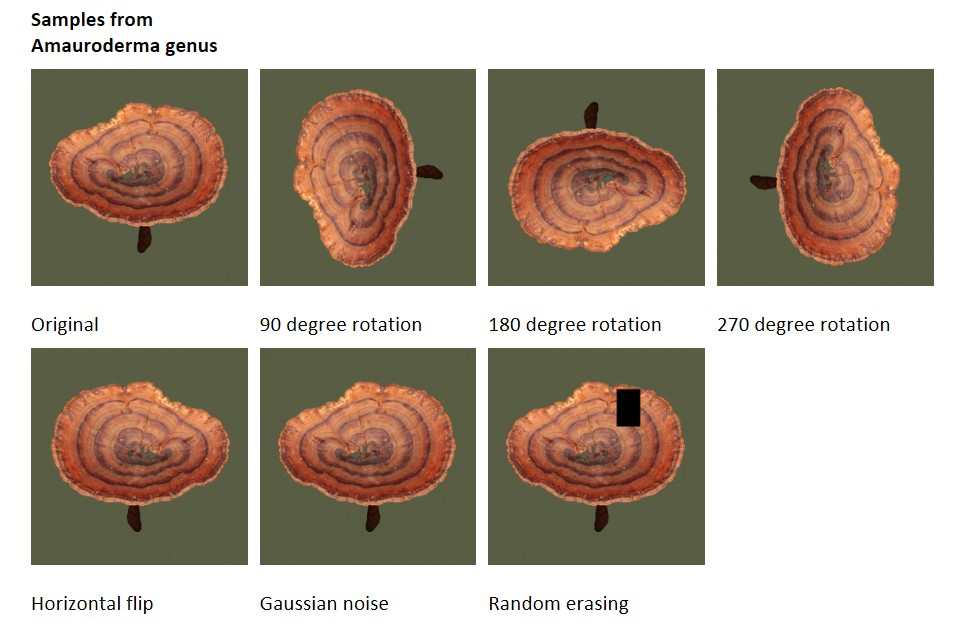
\includegraphics[width=0.9\textwidth]{figures/data_augmentation_example.jpg}
    \end{center}
    \caption{Data augmentation techniques applied to a sample image}
    \label{fig:augmentation}
\end{figure}
\FloatBarrier

\section{Architecture}
\label{sec:architecture}
Our primary model relies on two distinct sections: a non-tunable transfer learning section, and a tunable convolutional and fully-connected section. Our data pre-processing and model training pipeline is described in Figure \ref{fig:pipeline}.

We also use cross entropy loss, as it is a standard loss function for multi-class classification tasks. We also use a stochastic gradient optimizer, with a momentum of 0.8, weight decay of 0.001, and learning rate of 0.001. Our training flow uses 100 epochs with a batch size of 64.

\FloatBarrier
\begin{figure}[h]
    \begin{center}
    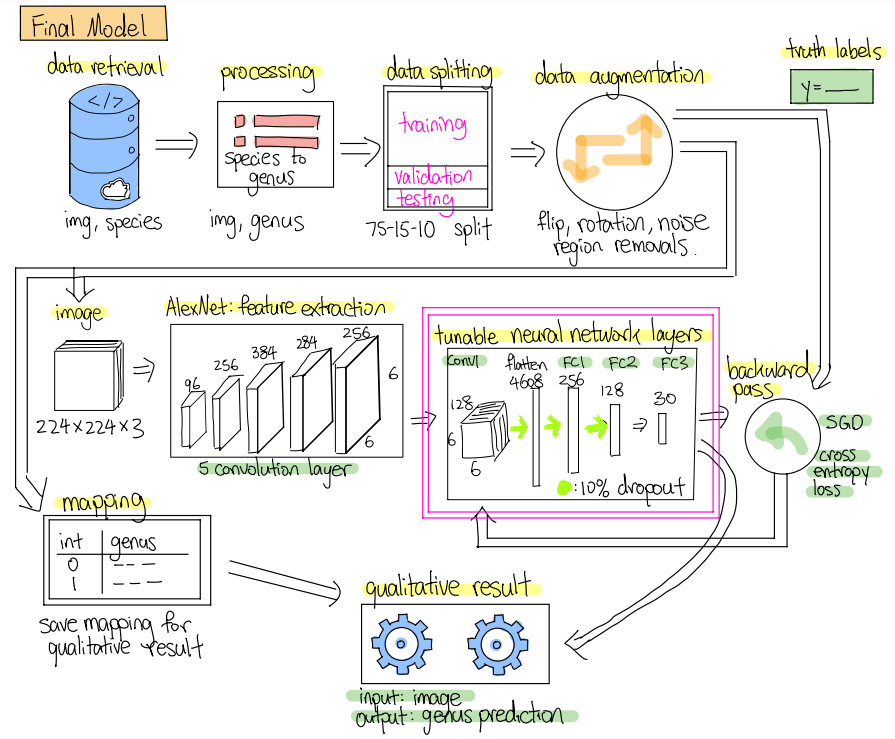
\includegraphics[width=0.9\textwidth]{figures/modelArchitecture_drawing.png}
    \end{center}
    \caption{Primary model processing and training pipeline}
    \label{fig:pipeline}
\end{figure}
\FloatBarrier

\subsection{Non-Tunable Section}
\label{sec:non_tunable_section}
We use AlexNet for high-level feature extraction, sourced from PyTorch's pre-trained models. AlexNet is a well-known convolutional architecture for image classification tasks \citep{NIPS2012_c399862d}. Since the model needs to differentiate between mushrooms with similar appearances, AlexNet excels in extracting the fine features that set them apart.

Its architecture is described in Figure \ref{fig:alexnet}. It processes a $3\times 244\times 244$ input image, and the feature extraction outputs a $256\times 6\times 6$ tensor. There are five convolutional layers and three pooling layers \citep{NIPS2012_c399862d}.

\FloatBarrier
\begin{figure}[h]
    \begin{center}
    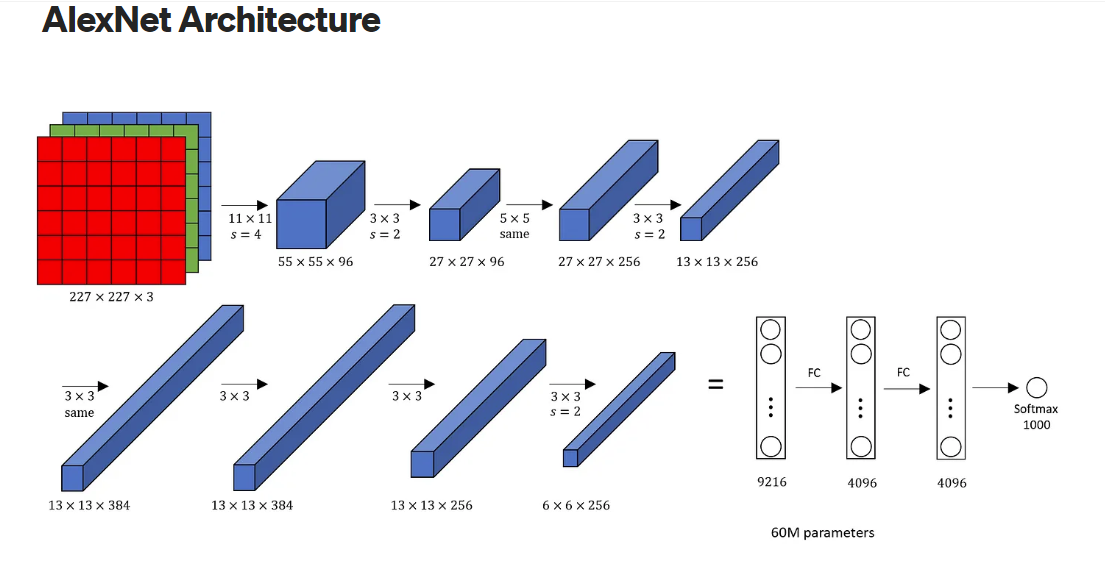
\includegraphics[width=0.9\textwidth]{figures/AlexNetStructure.png}
    \end{center}
    \caption{AlexNet architecture}
    \label{fig:alexnet}
\end{figure}
\FloatBarrier

\subsection{Tunable Section}
\label{sec:tunable_section}
To make the model specific to our team's project, we add an additional convolutional layer, which outputs a $128\times6\times6$ tensor. After this layer, the output is flattened and passed through three fully-connected layers with ReLU activation functions. The fully-connected layers have 256, 128, and 10 neurons, respectively, which matches the number of output classes in our dataset.

In total, there are $5+3$ layers in the non-tunable section, and $1+3$ layers in the tunable section, making our model architecture 12 layers in total.

\section{Baseline Model}
\label{sec:baseline}
Our baseline model is a random forests classifier trained with scikit-learn on the same dataset as our deep learning model. Decision tree classifiers, like random forests, are generally well-suited for multiclass problems \citep{GallRazaviEtAl.IntroductionRandomForests.2012}. We follow similar processing steps as the primary model, including a train-test split of 75\%-25\%, feature extraction, training, and evaluation. We do not apply data augmentation, as this benefits CNNs more.

We apply feature extraction on grayscale images with histogram of oriented gradients (HOG), an edge extraction descriptor algorithm \citep{N.DalalB.Triggs.HistogramsOrientedGradients.2005} and computed with scikit-image. As random forests does not automatically perform feature extraction (compared to deep convolutional networks), this step is done to provide the model with a more effective set of features to learn from. We compute HOG features on both the training and testing set with default parameters, in line with the process outlined by \cite{Dutta.RandomForestImage.2024}. We also use default hyperparameters for training, with the exception of the number of estimators, set to 500, which suggests is an optimal number of trees for increasing accuracy.

\section{Quantitative Results}
\label{sec:quantitative_results}

\section{Qualitative Results}
\label{sec:qualitative_results}

\section{Evaluation on New Data}
\label{sec:evaluation}

\section{Discussion}
\label{sec:discussion}

\section{Ethical Considerations}
\label{sec:ethics}
Many machine learning models rely on the "unauthorized uses of copyrighted" data for training purposes. This broadly results in infringement of the intellectual property rights and personal interests of the data owners \citep{Sobel.TaxonomyTrainingData.2021}. The dataset used in this project, MIND.Funga, is publicly licensed under a permissive copyleft license (CC BY NC 3.0) \citep{Drechsler-SantosKarstedtEtAl.MINDFunga.2023}. Images were sourced from contributions from the public and academics. However, the organizing project does not disclose that public contributions will be released under this license \citep{Drechsler-SantosKarstedtEtAl.MINDFunga.2023}, suggesting that the dataset may contain images that were not intended to be shared under this license as a result of inadequate informed consent.

The dataset also mostly contains images of tropical fungi from Brazil, with a small subset (approximately 500 out of 14 000) of the globally recorded number of fungi species \citep{LuckingAimeEtAl.UnambiguousIdentificationFungi.2020}. This results in a model that is primarily representative of Brazilian fungi species. As some fungi species can be poisonous, any practical real-world applications of our model may result in misclassifications, which may result in harm to users that rely on the model. This is a significant ethical concern, as the model may be used by individuals who are not experts in mycology, and may not be able to identify the potential risks of consuming certain fungi species.

\label{last_page}

\bibliography{final_report}
\bibliographystyle{iclr2022_conference}

\end{document}
